

\tikzset{every picture/.style={line width=0.75pt}} %set default line width to 0.75pt        

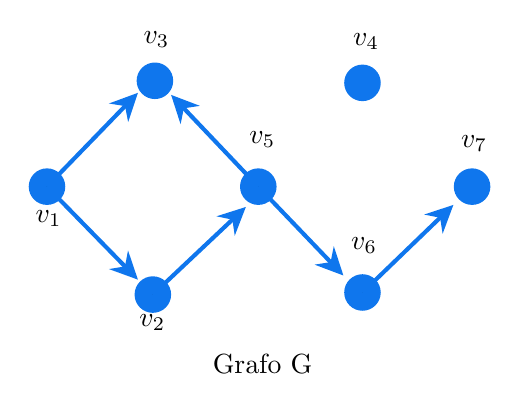
\begin{tikzpicture}[x=0.75pt,y=0.75pt,yscale=-1,xscale=1]
%uncomment if require: \path (0,182); %set diagram left start at 0, and has height of 182

%Shape: Circle [id:dp5077982020192706] 
\draw  [draw opacity=0][fill={rgb, 255:red, 15; green, 118; blue, 237 }  ,fill opacity=1 ] (17,76.81) .. controls (17,71.94) and (20.94,68) .. (25.81,68) .. controls (30.67,68) and (34.61,71.94) .. (34.61,76.81) .. controls (34.61,81.67) and (30.67,85.61) .. (25.81,85.61) .. controls (20.94,85.61) and (17,81.67) .. (17,76.81) -- cycle ;
%Shape: Circle [id:dp7144769570638401] 
\draw  [draw opacity=0][fill={rgb, 255:red, 15; green, 118; blue, 237 }  ,fill opacity=1 ] (68,128.81) .. controls (68,123.94) and (71.94,120) .. (76.81,120) .. controls (81.67,120) and (85.61,123.94) .. (85.61,128.81) .. controls (85.61,133.67) and (81.67,137.61) .. (76.81,137.61) .. controls (71.94,137.61) and (68,133.67) .. (68,128.81) -- cycle ;
%Shape: Circle [id:dp10535612642783376] 
\draw  [draw opacity=0][fill={rgb, 255:red, 15; green, 118; blue, 237 }  ,fill opacity=1 ] (69,25.81) .. controls (69,20.94) and (72.94,17) .. (77.81,17) .. controls (82.67,17) and (86.61,20.94) .. (86.61,25.81) .. controls (86.61,30.67) and (82.67,34.61) .. (77.81,34.61) .. controls (72.94,34.61) and (69,30.67) .. (69,25.81) -- cycle ;
%Shape: Circle [id:dp8289908753476658] 
\draw  [draw opacity=0][fill={rgb, 255:red, 15; green, 118; blue, 237 }  ,fill opacity=1 ] (118.81,76.81) .. controls (118.81,71.94) and (122.75,68) .. (127.61,68) .. controls (132.47,68) and (136.42,71.94) .. (136.42,76.81) .. controls (136.42,81.67) and (132.47,85.61) .. (127.61,85.61) .. controls (122.75,85.61) and (118.81,81.67) .. (118.81,76.81) -- cycle ;
%Shape: Circle [id:dp06972249328365487] 
\draw  [draw opacity=0][fill={rgb, 255:red, 15; green, 118; blue, 237 }  ,fill opacity=1 ] (169,127.81) .. controls (169,122.94) and (172.94,119) .. (177.81,119) .. controls (182.67,119) and (186.61,122.94) .. (186.61,127.81) .. controls (186.61,132.67) and (182.67,136.61) .. (177.81,136.61) .. controls (172.94,136.61) and (169,132.67) .. (169,127.81) -- cycle ;
%Shape: Circle [id:dp7147960092743524] 
\draw  [draw opacity=0][fill={rgb, 255:red, 15; green, 118; blue, 237 }  ,fill opacity=1 ] (221.81,76.81) .. controls (221.81,71.94) and (225.75,68) .. (230.61,68) .. controls (235.47,68) and (239.42,71.94) .. (239.42,76.81) .. controls (239.42,81.67) and (235.47,85.61) .. (230.61,85.61) .. controls (225.75,85.61) and (221.81,81.67) .. (221.81,76.81) -- cycle ;
%Shape: Circle [id:dp469938637266508] 
\draw  [draw opacity=0][fill={rgb, 255:red, 15; green, 118; blue, 237 }  ,fill opacity=1 ] (169,26.81) .. controls (169,21.94) and (172.94,18) .. (177.81,18) .. controls (182.67,18) and (186.61,21.94) .. (186.61,26.81) .. controls (186.61,31.67) and (182.67,35.61) .. (177.81,35.61) .. controls (172.94,35.61) and (169,31.67) .. (169,26.81) -- cycle ;
%Straight Lines [id:da4397858754948907] 
\draw [color={rgb, 255:red, 15; green, 118; blue, 237 }  ,draw opacity=1 ][fill={rgb, 255:red, 0; green, 0; blue, 0 }  ,fill opacity=1 ][line width=1.5]    (25.81,76.81) -- (66.83,34.48) ;
\draw [shift={(69.61,31.61)}, rotate = 494.1] [fill={rgb, 255:red, 15; green, 118; blue, 237 }  ,fill opacity=1 ][line width=0.08]  [draw opacity=0] (13.4,-6.43) -- (0,0) -- (13.4,6.44) -- (8.9,0) -- cycle    ;
%Straight Lines [id:da7612336938851023] 
\draw [color={rgb, 255:red, 15; green, 118; blue, 237 }  ,draw opacity=1 ][fill={rgb, 255:red, 0; green, 0; blue, 0 }  ,fill opacity=1 ][line width=1.5]    (127.61,76.81) -- (88.37,35.51) ;
\draw [shift={(85.61,32.61)}, rotate = 406.46000000000004] [fill={rgb, 255:red, 15; green, 118; blue, 237 }  ,fill opacity=1 ][line width=0.08]  [draw opacity=0] (13.4,-6.43) -- (0,0) -- (13.4,6.44) -- (8.9,0) -- cycle    ;
%Straight Lines [id:da521868726384179] 
\draw [color={rgb, 255:red, 15; green, 118; blue, 237 }  ,draw opacity=1 ][fill={rgb, 255:red, 0; green, 0; blue, 0 }  ,fill opacity=1 ][line width=1.5]    (25.81,76.81) -- (66.81,118.75) ;
\draw [shift={(69.61,121.61)}, rotate = 225.64] [fill={rgb, 255:red, 15; green, 118; blue, 237 }  ,fill opacity=1 ][line width=0.08]  [draw opacity=0] (13.4,-6.43) -- (0,0) -- (13.4,6.44) -- (8.9,0) -- cycle    ;
%Straight Lines [id:da3551036263203664] 
\draw [color={rgb, 255:red, 15; green, 118; blue, 237 }  ,draw opacity=1 ][fill={rgb, 255:red, 0; green, 0; blue, 0 }  ,fill opacity=1 ][line width=1.5]    (76.81,128.81) -- (118.7,89.35) ;
\draw [shift={(121.61,86.61)}, rotate = 496.72] [fill={rgb, 255:red, 15; green, 118; blue, 237 }  ,fill opacity=1 ][line width=0.08]  [draw opacity=0] (13.4,-6.43) -- (0,0) -- (13.4,6.44) -- (8.9,0) -- cycle    ;
%Straight Lines [id:da5375483437520805] 
\draw [color={rgb, 255:red, 15; green, 118; blue, 237 }  ,draw opacity=1 ][fill={rgb, 255:red, 0; green, 0; blue, 0 }  ,fill opacity=1 ][line width=1.5]    (127.61,76.81) -- (165.84,116.72) ;
\draw [shift={(168.61,119.61)}, rotate = 226.23] [fill={rgb, 255:red, 15; green, 118; blue, 237 }  ,fill opacity=1 ][line width=0.08]  [draw opacity=0] (13.4,-6.43) -- (0,0) -- (13.4,6.44) -- (8.9,0) -- cycle    ;
%Straight Lines [id:da8162139572767808] 
\draw [color={rgb, 255:red, 15; green, 118; blue, 237 }  ,draw opacity=1 ][fill={rgb, 255:red, 0; green, 0; blue, 0 }  ,fill opacity=1 ][line width=1.5]    (177.81,127.81) -- (218.73,88.38) ;
\draw [shift={(221.61,85.61)}, rotate = 496.07] [fill={rgb, 255:red, 15; green, 118; blue, 237 }  ,fill opacity=1 ][line width=0.08]  [draw opacity=0] (13.4,-6.43) -- (0,0) -- (13.4,6.44) -- (8.9,0) -- cycle    ;

% Text Node
\draw (18.82,86.72) node [anchor=north west][inner sep=0.75pt]    {$v_{1}$};
% Text Node
\draw (68.82,136.72) node [anchor=north west][inner sep=0.75pt]    {$v_{2}$};
% Text Node
\draw (70.82,0.72) node [anchor=north west][inner sep=0.75pt]    {$v_{3}$};
% Text Node
\draw (171.82,1.72) node [anchor=north west][inner sep=0.75pt]    {$v_{4}$};
% Text Node
\draw (121.82,48.72) node [anchor=north west][inner sep=0.75pt]    {$v_{5}$};
% Text Node
\draw (170.82,99.72) node [anchor=north west][inner sep=0.75pt]    {$v_{6}$};
% Text Node
\draw (223.82,50.72) node [anchor=north west][inner sep=0.75pt]    {$v_{7}$};
% Text Node
\draw (104.17,156.29) node [anchor=north west][inner sep=0.75pt]   [align=left] {Grafo G};


\end{tikzpicture}